\section{Rendering}
	
	\begin{frame}[plain, c]
		
	\begin{center}
		\Huge Rendering
	\end{center}
	
	\begin{figure}
				\centering
				\begin{minipage}{.4\paperwidth}
					\centering
					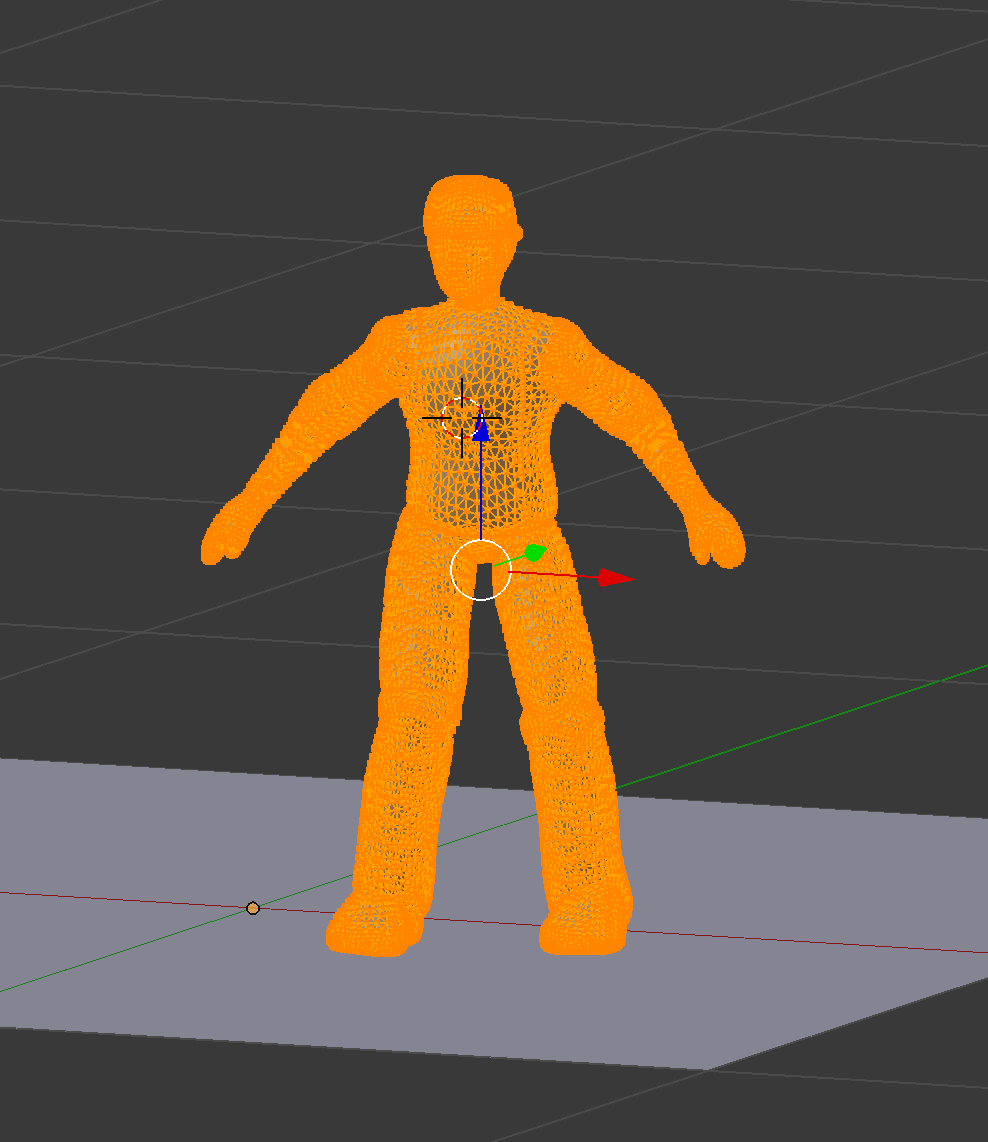
\includegraphics[width=.3\paperwidth]{02_Rendering/img/triangulars.png}
				\end{minipage}%
				\begin{minipage}{.4\paperwidth}
					\centering
					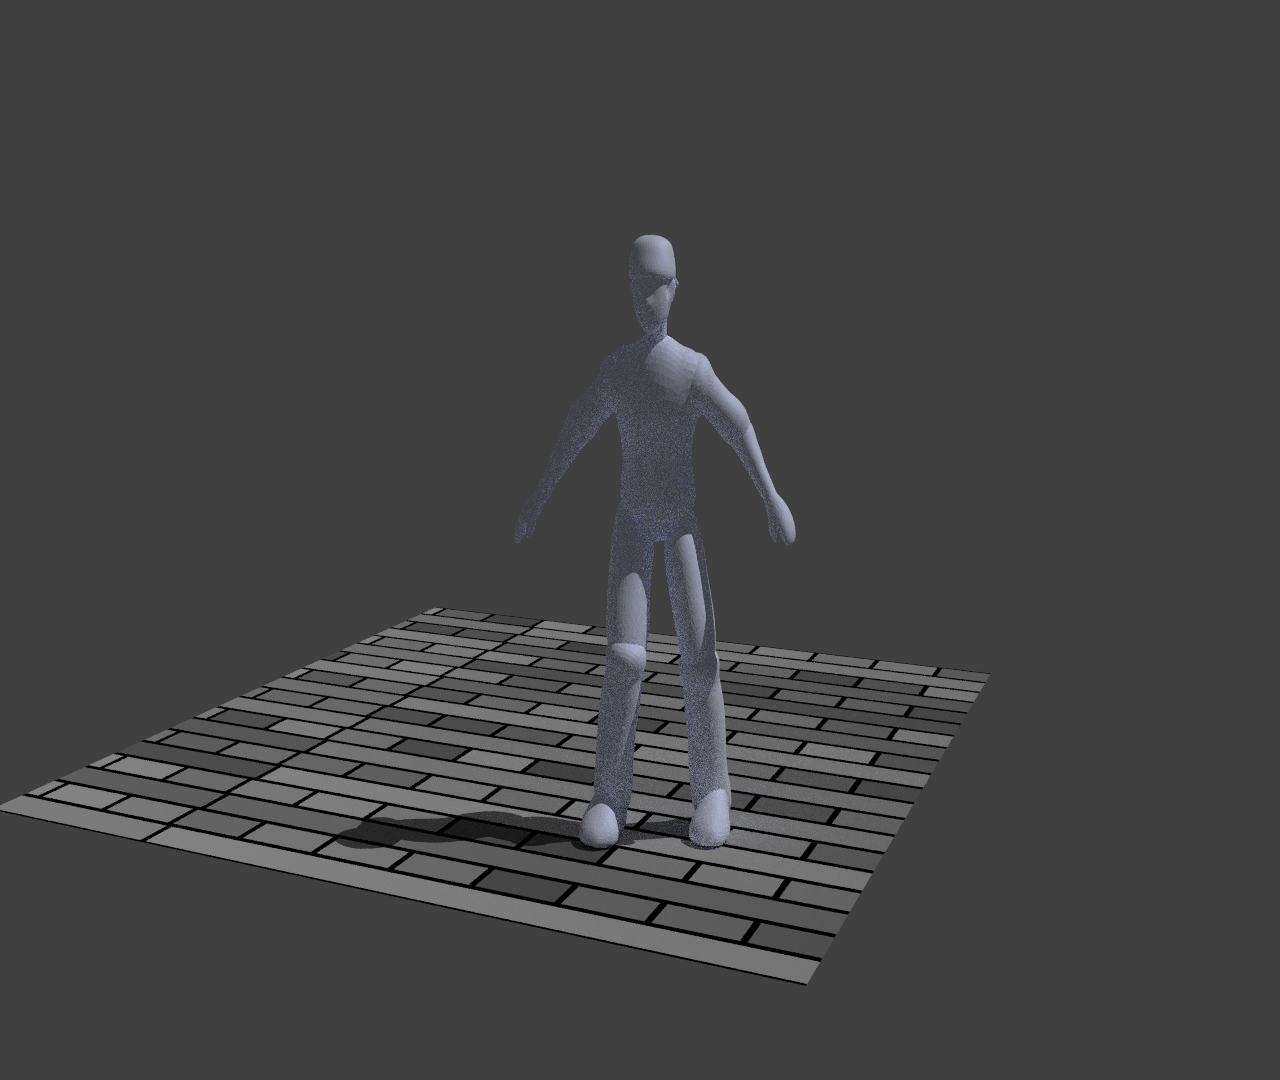
\includegraphics[width=.4\paperwidth]{02_Rendering/img/rendered.png}
				\end{minipage}
		\end{figure}

		
	\end{frame}
	\pdfnote{Whatever}
	\pdfnote{zrdz}
	\pdfnote{zrdz}
	\pdfnote{zrdz}
	\pdfnote{zrdz}
	

		
		% Commands to include a figure:
		%\begin{figure}
		%\includegraphics[width=\textwidth]{your-figure's-file-name}
		%\caption{\label{fig:your-figure}Caption goes here.}
		%\end{figure}
		
	
	\begin{frame}{\Huge{Rendering in der Praxis}}
		
		\begin{figure}
				\centering
				\begin{minipage}{.4\paperwidth}
					\centering
					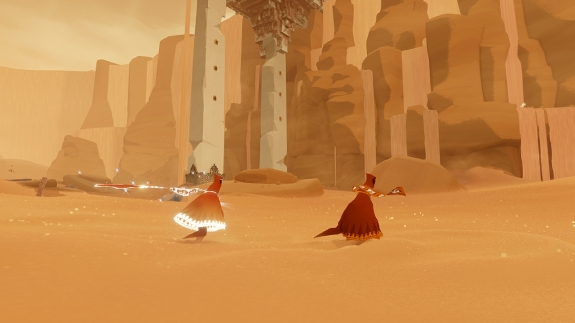
\includegraphics[width=.4\paperwidth]{02_Rendering/img/journey.jpg}
				\end{minipage}%
				\begin{minipage}{.5\paperwidth}
					\centering
					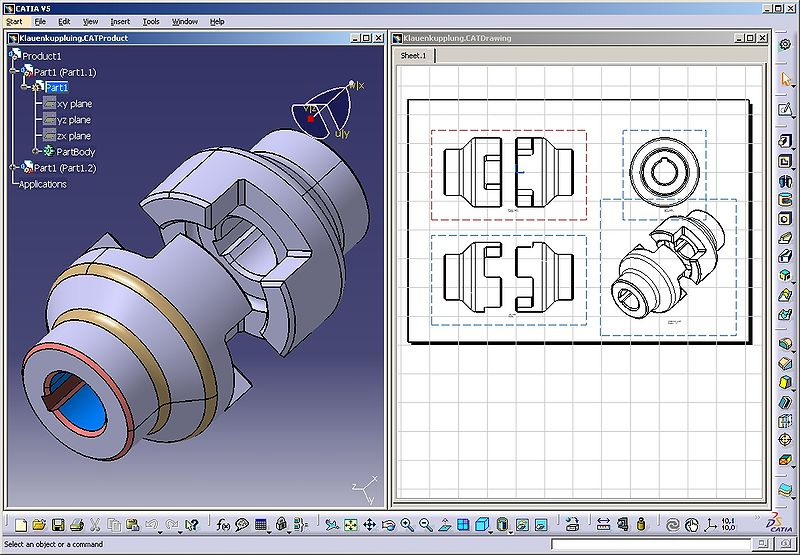
\includegraphics[width=.4\paperwidth]{02_Rendering/img/cad.jpg}
				\end{minipage}
		\end{figure}
		
		\blfootnote{Bildquellen: \cite{journey, cad}}
		
\end{frame}
	
\begin{frame}{\Huge{Rendering im Film}}
		
		\begin{figure}
				\centering
					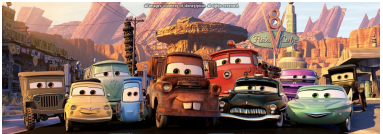
\includegraphics[width=.8\paperwidth]{02_Rendering/img/cars.png}
				\centering
		\end{figure}
		
		\begin{itemize}
			\item Komplexe Szenen
			\item Viele Lichtquellen
			\item 24 Bilder pro Sekunde
		\end{itemize}
		
		\blfootnote{Bildquellen: \cite{cars}}
	\end{frame}
	
	\subsubsection{Licht}
	
\begin{frame}{\Huge{Licht}}
		
		\begin{figure}
				\centering
					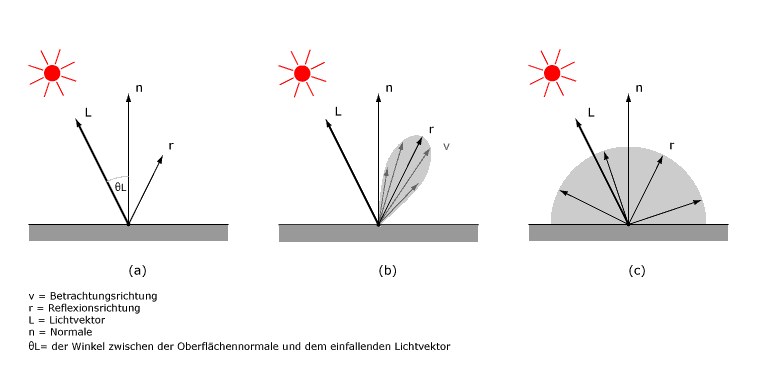
\includegraphics[width=.8\paperwidth]{02_Rendering/img/reflexion.png}
				\centering
		\end{figure}
		
		\begin{itemize}
			\item Ideale spekulare Reflexion
			\item Reale spekulare Reflexion
			\item Diffuse Reflexion
		\end{itemize}
		
		\blfootnote{Bildquellen: \cite{reflexion}}
	\end{frame}
	
	\begin{frame}{\colorbox{black!10}{\Huge{Materialien}}}
		
		\begin{figure}
				\centering
					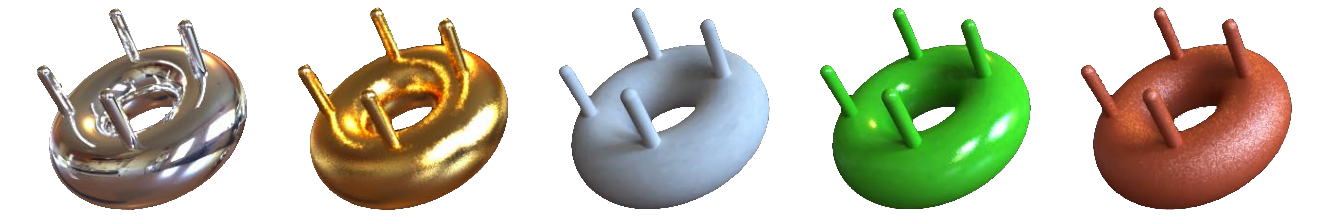
\includegraphics[width=.8\paperwidth]{02_Rendering/img/materials.png}
				\centering
		\end{figure}
		
		\blfootnote{Bildquellen: \cite{realImages}}
	\end{frame}
	
\begin{frame}{\Huge{Lokale Reflexionsmodelle}}
		
		  \begin{tabular}{cl}  
         \begin{tabular}{c}
           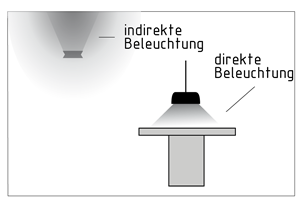
\includegraphics[height=3cm, width=3cm]{02_Rendering/img/directLight.png}
           \end{tabular}
           & \begin{tabular}{l}
             \parbox{0.6\linewidth}{%  change the parbox width as appropiate
             \textbf{Bi-Directional Reflection Distribution Function(BRDF)}
             

$$\mathrm{BRDF}=f(\theta_\mathrm{in}, \phi_\mathrm{in}, \theta_\mathrm{ref}, \phi_\mathrm{ref}) = f(\vec{\omega_{i}}, \vec{\omega_{o}})$$
   
    }
         \end{tabular}  \\
\end{tabular}
		
		\blfootnote{Bildquellen: \cite{directLight}}
\end{frame}
	
\begin{frame}{\Huge{Lambertsche Reflexion}}
		
		  \begin{tabular}{cl}  
         \begin{tabular}{c}
           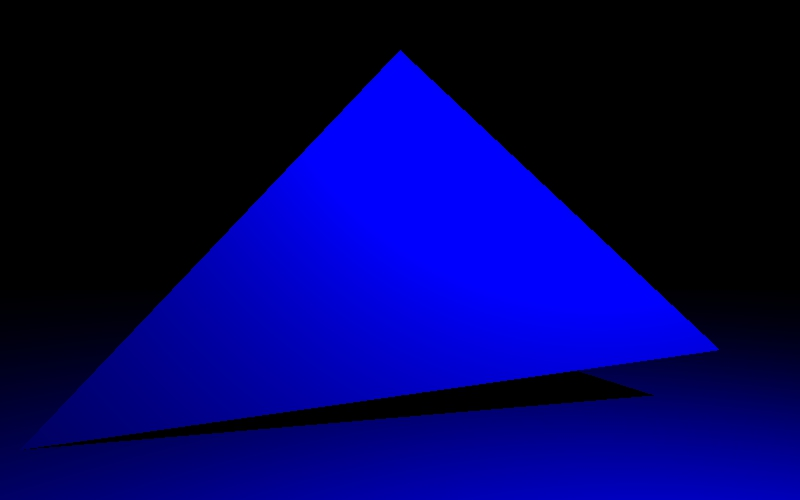
\includegraphics[width=5cm]{02_Rendering/img/lambertian.jpg}
           \end{tabular}
           & \begin{tabular}{l}
             \parbox{0.4\linewidth}{%  change the parbox width as appropiate            

$$I_{D} =\vec{\omega_{i}} \cdot \vec{n}CI_{L}$$


   
    }
         \end{tabular}  \\
\end{tabular}
\end{frame}

\begin{frame}{\Huge{Blinn-Phong BRDF}}
		
		\begin{figure}
				\centering
				\begin{minipage}{.4\paperwidth}
					\centering
					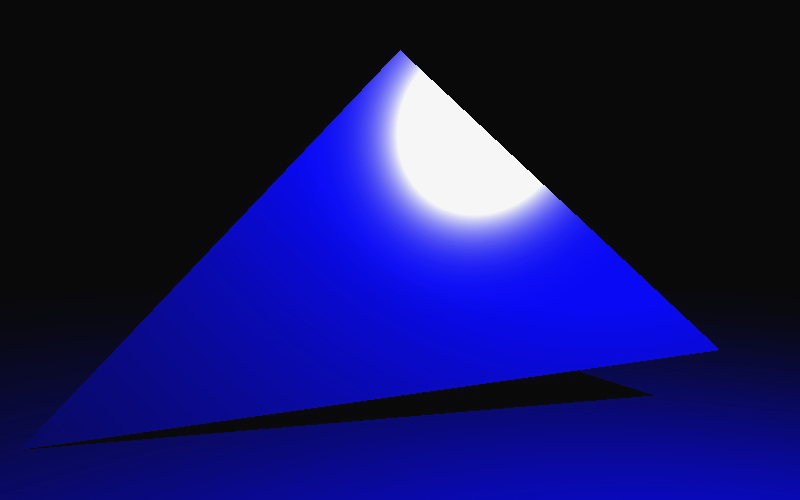
\includegraphics[width=.4\paperwidth]{02_Rendering/img/glossy.jpg}
				\end{minipage}%
				\begin{minipage}{.5\paperwidth}
					\centering
					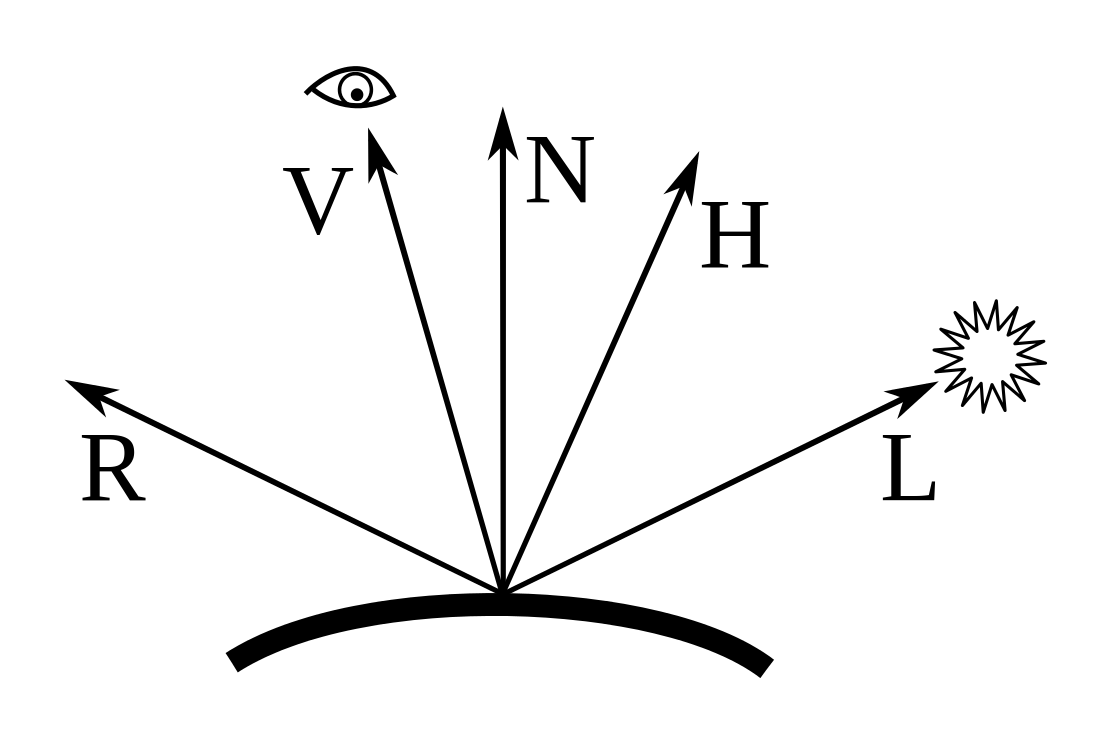
\includegraphics[width=.4\paperwidth]{02_Rendering/img/h.png}
				\end{minipage}
		\end{figure}
		
    

$$f_{s}(\vec{\omega_{i}}, \vec{\omega_{o}})=\frac{k_{L}}{\pi} + k_{G}\frac{8 + s}{8\pi}z^s$$  $$\mathrm{\quad mit\quad}z=\max(0,\vec{h} \cdot \vec{n})$$
$$\mathrm{\quad mit\quad}\vec{h}=\frac{\vec{\omega_{i}} + \vec{\omega_o}}{2}$$

		\blfootnote{Bildquellen: \cite{h}}  

\end{frame}

\begin{frame}{\Huge{Globale Beleuchtungsmodelle}}
		
		\begin{figure}
				\centering
					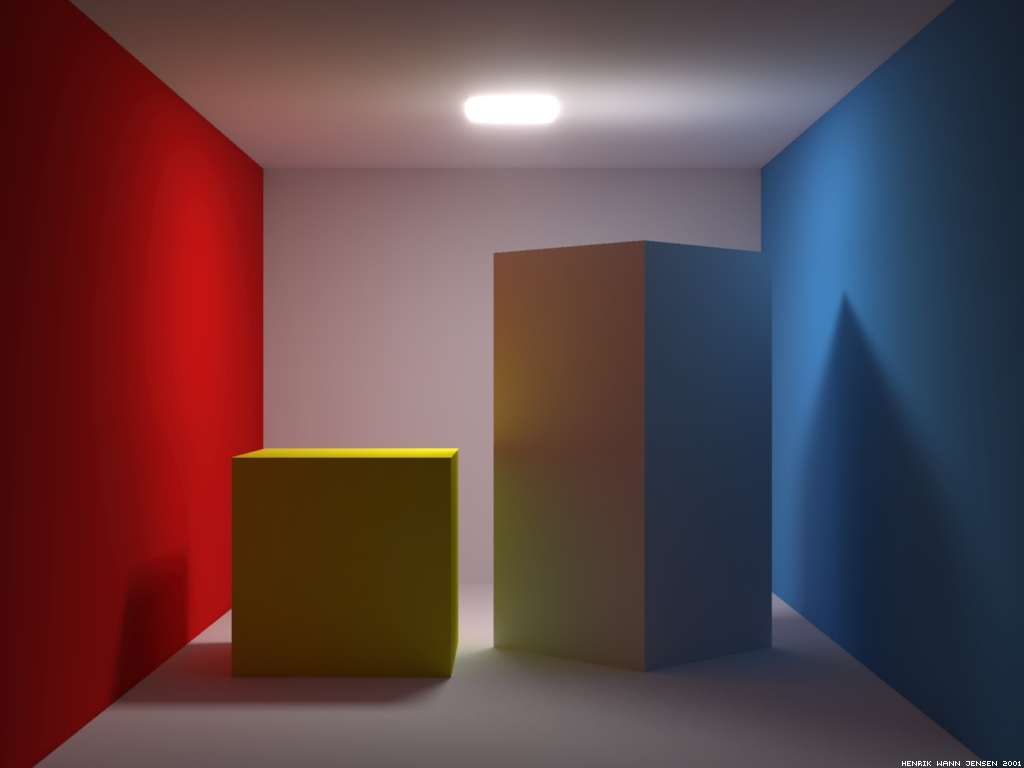
\includegraphics[width=.8\paperwidth]{02_Rendering/img/cornellbox.jpg}
				\centering
		\end{figure}

		\blfootnote{Bildquellen: \cite{cornell}}  

\end{frame}
